\documentclass[10pt]{article}


\usepackage[utf8x]{inputenc}

\usepackage[frenchb]{babel}
\usepackage{amsmath}
\usepackage{amssymb}
\usepackage{amsfonts}
\usepackage{color}
\usepackage{caption}
\usepackage{easytable}
\usepackage{epsfig}
\usepackage{etex}
\usepackage{etoolbox}
\usepackage{here}
\usepackage{layout} % \layout au début de doc -> longueurs caractéristiques de la mise en page
\usepackage{makeidx}
\usepackage{mathrsfs}
\usepackage{mathtools}
%\usepackage{nopageno}
\usepackage{pslatex}
\usepackage{pstricks}
\usepackage{pstricks-add}
\usepackage[retainorgcmds]{IEEEtrantools} % des beaux tableaux (équations, matrice etc...) cf rapport TIPE
\usepackage{wrapfig}
\usepackage{lmodern}
\usepackage{eurosym}
\usepackage{csvsimple}
\usepackage{tikz}
\usepackage{float}
\usepackage{pgfplots}
\usepackage{siunitx}
\sisetup{
unitsep = \cdot,
decimalsymbol = comma,
expproduct = \cdot
}

\usepackage[coverpage,fancysections]{polytechnique}
\titleformat{\chapter}[hang]{\Huge\bfseries\sffamily}{\LARGE}{0em}{}[]
\title{Il dit qu'il voit pas le rapport}
\subtitle{Sexuel le rapport, sexuel.}
\author{ Vincent \textsc{Dufour-Descieux} \\ Odilon \textsc{Formery} \\ Ahmed \textsc{Krarti} \\ Louis \textsc{Legrand} \\ Augustin \textsc{Lenormand} \\   Camille \textsc{Masset} }
\begin{document}

\maketitle

\section{Contexte et donn1ées}

	\subsection{Enjeux et probl\'ematique}
	
		Dans cette partie, nous allons tout d’abord détailler la distribution grande échelle de l’électricité dans le but de comprendre les enjeux de l’étude qui va suivre. Celle-ci est motivée par le fait que la répartition de cette distribution n’est pas éparpillée tout au long de la journée mais dans des périodes précises qui sont les pics de consommation que nous étudierons ensuite. La solution proposée par GDF Suez concernant les pics de consommation, est le Smart Grid, nous le détaillerons dans une troisième partie. Celui-ci peut être complété par un système qui s’appelle l’agrégateur de flexibilité et qui sera détaillé après. Enfin nous replacerons notre PSC dans ce contexte.
	
		
		\subsubsection{Distribution de l'électricité}
		
			Le prix de l'électricité, celui que les français peuvent lire sur leur facture, est composé de quatre parties (chiffres moyens en 2013) :
			\begin{itemize}
				\item la production (31\%) ;
				\item l'acheminement par le gestionnaire de réseau (30\%) ;
				\item la commercialisation par le fournisseur (8\%) ;
				\item les taxes et la contribution au service public de l'électricité (31\%).
			\end{itemize}
			
			Précisons ce qui se cache derrière ces parties.
			La production est l'étape de transformation des sources d'énergie en électricité.
			En France, la principale source d'énergie est le nucléaire (78\%). Viennent ensuite les sources thermiques (charbon, gaz) et hydrauliques (9\% chacune), puis les énergies renouvelables intermittentes (éolien: 2\%, photovoltaïque: 1\%) ou continue (géothermie: 1\%).
			
			Le nucléaire, l'hydraulique et la géothermie permettent une production continue (avec des ajustements possibles pour les barrages hydroélectriques), et constituent donc une base solide pour la production électrique en France. Les sources thermiques sont essentiellement utilisées en période de forte consommation, car il est très rapide de mettre en fonctionnement une centrale à charbon par exemple, mais de telles centrales sont très polluantes (rejet de gaz à effet de serre dans l'atmosphère). Les autres sources d'énergie produisent en fonction des conditions climatiques (soleil, vent) et sont donc moins fiables. En particulier, on ne peut pas s'appuyer sur de telles sources d'énergies pour faire face à un pic de consommation.
			
			L'acheminement consiste à amener l'électricité depuis la centrale de production vers le consommateur final. On peut décomposer cet acheminement en deux parties : le transport (lignes à haute et très haute tension) et la distribution (lignes à moyenne et basse tension). Les gestionnaires de réseaux d'électricité sont chargés de l'entretien et du bon fonctionnement des réseaux (sécurité, dépannage, qualité, relevé des compteurs). Ils sont rémunérés par le Tarif d'Utilisation des Réseaux Publics d'Électricité (TURPE), fixé par l'État. Les gestionnaires de réseaux sont RTE pour le transport et ERDF et les ELD (Entreprises Locales de Distribution) pour la distribution.
			
			La commercialisation est assurée par le fournisseur qui est le contact privilégié du client. Il est aussi en relation avec les gestionnaires de réseaux de distributions. Il répercute les prix de l'acheminement et les taxes dans ses tarifs. Le consommateur peut choisir entre des prix réglementés fixés par les pouvoirs publics et proposés par les distributeurs historiques (comme EDF) ou une offre à prix de marché (contrat).
			
			L'électricité est soumise à quatre taxes fixées par les pouvoirs publics : la TVA, la Contribution au Service Public de l'Électricité (CSPE), la Taxe sur la Consommation Finale d'Électricité (TCFE) et la Contribution Tarifaire d'Acheminement (CTA). La CSPE permet essentiellement d'investir dans le développement des énergies renouvelables et de financer le surcoût de la production d'électricité dans les zones non connectées au réseau continental. La TCFE est perçue par les communes et les départements et permet de financer les travaux sur les installations électriques locales. La CTA finance partiellement les retraites des salariés des gestionnaires de transport.
			Les fournisseurs rencontrent des difficultés à répondre à la demande des clients pendant certaines périodes : les pics de consommation.
		
		
		\subsubsection{Pic de consommation}
			Une pointe de consommation électrique est la consommation la plus élevée sur un réseau électrique. Elle peut résulter de plusieurs facteurs : temporels (heure de pointe), climatiques (forte chaleur, températures trop basses), ...
			
			On en distingue trois types majeurs :
			
			\begin{itemize}
				\item les pointes journalières qui se produisent souvent en fin de journée un jour de semaine, lorsque les personnes rentrent du travail; la pointe sera plus accentuée dans les réseaux où le chauffage de l'eau et les appareils électroménagers utilisent l'électricité plutôt que le gaz;
				\item les pointes saisonnières peuvent survenir en été ou en hiver (cas de la France), mais dans les deux cas, les températures extrêmes influent sur la demande de climatisation ou de chauffage électrique des ménages;
				\item certaines pointes sont aussi causées par les infrastructures d'utilités publiques telles que l'éclairage public, le transport ferroviaire, etc.
			\end{itemize}
			
			La situation de la France est la suivante : la pointe progresse  plus vite que la consommation électrique : elle augmente de 3\%, alors que, dans le même temps, la consommation électrique connaît une hausse de 0,6\%. Plusieurs raisons en sont à l'origine, notamment la place du chauffage électrique et le développement de nouveaux usages de l'électricité (équipements électroménagers, informatiques, recharges multiples). Il est donc nécessaire d'agir rapidement pour lutter contre ces pics de consommation qui coûtent cher et ont un impact environnemental au travers des augmentations d'émission de CO$_2$.
			Par exemple, la perte d'un degré de température se traduit en France en 2012 par une augmentation estimée d'électricité de 2300~MW contre 600~MW en Grande-Bretagne.
			
			Quels sont les solutions pour gérer ces pics ? Plusieurs moyens sont mis en œuvre par les gestionnaires de réseau.
			La solution la plus évidente et la plus ancienne consistait en l'augmentation de la capacité de production par le biais de construction de nouvelles infrastructures de production, de transport et de distribution. Mais cette solution a très vite atteint ces limites d'une part car elle présente des risques environnementaux (émission de CO$_2$) mais aussi des risques de blackout dues à la surcharge d'alimentation.
			Une autre solution consiste à baisser le niveau de la consommation en commandant à un opérateur dit \og d'effacement \fg~la coupure immédiate et coordonnée de certains postes de consommation, tout cela est géré par des réseaux intelligents : les \textit{Smart Grids}.
		
			
		\subsubsection{Les \emph{Smart Grids}}
		
			L'effacement résidentiel consiste à réduire temporairement la consommation d'électricité d'un grand nombre de petits sites, en particulier de logements, de façon à diminuer la demande. Il s'agit par exemple d'interrompre brièvement, mais de façon synchronisée, l'alimentation de radiateurs ou climatiseurs situés dans des logements pour, au total, réduire la consommation d'électricité d'une région ou du pays.
			
			Cela se matérialise par la mise en place d'un boîtier (Linky) qui s'installe sur le tableau électrique et qui permet de mesurer et commander certains usages en temps réel (par exemple, chauffe-eau et radiateurs). Un système d'information complète le tout en recueillant les données et générant les ordres de modulation. Le pilotage est opéré à distance par un opérateur et ne requiert aucune action directe des utilisateurs qui souscrivent à ce service. Un consommateur qui dispose d'une offre d'effacement se verra ainsi rémunéré pour le service qu'il apporte au système électrique
			
			Avec le développement des nouvelles technologies, les gestionnaires du réseau (EDF, RTE, ERDF) ont mis à profit ces TICS pour moderniser leurs réseaux de distribution. Ces réseaux intelligents, les Smarts Grids, permettent de déconnecter des appareils électriques non primordiaux lors de fortes demandes en électricité. Ce nouveau réseau sert avant tout à limiter les risques d'apparition de pointes importantes de consommation électrique et maintenir une fourniture d'électricité efficace, durable, économique et sécurisée.
			
			Ces Smarts Grids permettent de tenir compte de la variabilité des sources de production d'électricité renouvelable, c'est-à-dire leur fluctuation en fonction des contraintes météorologiques (ensoleillement, vents, etc.), ainsi que l'augmentation de la production dite décentralisée (parc éolien raccordé au réseau de distribution ou consommateur final disposant de panneaux photovoltaïques sur le toit de son habitat qui devient producteur d'énergie par exemple) et les ambitions de réduction des consommations d'énergie complexifient la gestion de l'équilibre entre production et consommation. En favorisant l'intégration des productions d'électricité à partir d'énergies de sources renouvelables, les Smart grids ont un impact fort sur la réduction d'émission de CO$_2$.
			
			Les effets de ces Smart Grids peuvent être développés grâce à un agrégateur de flexibilité que nous allons maintenant étudier.
		
		
		\subsubsection{L'agrégateur de flexibilité}
		
			L’agrégateur est une prestation complémentaire, un intermédiaire entre le système électrique et ses utilisateurs. Il crée de la valeur pour ses clients en revendant de la flexibilité au système électrique, ce que l'on qualifie parfois de \og centrale électrique virtuelle \fg. Pour que tout cela fonctionne, il faut stocker de l’énergie pendant les périodes creuses pour pouvoir faire face aux pics. Ce stockage se fait au niveau :
			
			\begin{itemize}
				\item individuel : grâce aux batteries des VE, ballon d'eau chaude ;
				\item des bâtiments : inertie thermique, batterie chaude ou froide ;
				\item des collectivités : barrage électrique, château d'eau ;
				\item industriel : stockage de produits intermédiaires (cimenterie).
			\end{itemize}
			
			Cela nécessite :
	
			\begin{itemize}
				\item de rendre les immeubles et  les sites industriels qu'il pilote \og intelligents \fg~ ;
				\item de modèles pour prévoir les résultats de son action ;
				\item d'informations pour anticiper les évolutions du marché.
			\end{itemize}
			
			Malheureusement tout cela est assez lent à se mettre en place pour plusieurs raisons : la loi NOME ne permet pas la mise en place de ces réseaux avant 2016, de plus le consommateur doit avoir la possibilité de revenir en mode \og normal \fg~ à tout moment, des études sur le comportement des utilisateurs doivent être faites pour pouvoir choisir les moments où effacer l’électricité ou non.
	
		\subsubsection{Notre PSC et son inscription dans ce contexte}
		
			Des solutions au problème des pics de consommation ont été apportées à travers les Smart Grids et l’agrégateur de flexibilité, cependant ces deux systèmes ont besoin d’informations sur la consommation d’électricité des clients pour soit effacer la consommation à travers les Smart Grids, soit pour savoir quand l’agrégateur devra redistribuer l’énergie accumulée. Les fournisseurs, tels que GDF Suez, peuvent obtenir cela pour les habitudes actuelles car la consommation d’électricité vient principalement de l’électroménager, de la lumière, du chauffage. Mais un changement commence à s’opérer dans le quotidien des individus et il s’agit de la voiture électrique. En effet, celle-ci va amener des consommations supplémentaires d’électricité à travers sa recharge et prévoir comment cela va influer sur les pics de consommation mérite une étude poussée. C’est là qu’intervient notre PSC : nous allons étudier le comportement des utilisateurs de véhicules électriques pour savoir quand est-ce qu’ils rechargeront leur véhicule et quel effet cela aura-t-il sur le réseau. GDF Suez souhaite aussi gérer intelligemment l’augmentation des pics de consommation dus aux véhicules électriques en apportant une nouvelle idée : lorsque le véhicule sera branché il sera possible de ne pas le recharger pour repousser l’utilisation d’énergie à un moment où le réseau sera moins demandé ou même de fournir de l’énergie au réseau pour que l’effet bénéfique soit amplifié. Nous tenterons de prévoir le nombre de personnes intéressés par cette offre et comment elle influera sur le réseau au cours de notre étude.
			
			
	
	\subsection{Données collectées}
	
		Nous avons donc cherché des informations sur le comportement des utilisateurs de véhicules électriques que nous analyserons ensuite. Malheureusement, puisque leur nombre est aujourd’hui peu conséquent (environ 30000) il est difficile de trouver des études dessus. Nous avons cependant réussi à en réunir quelques-unes :
		
		\begin{itemize}
			\item une étude du Club Alsace Voiture Electrique sur les habitudes de ces utilisateurs. L’enquête est intéressante et nous donne des informations (fréquence des recharges des voitures, lieu d’utilisation des bornes…) et on peut la considérer comme représentative car elle a été faite auprès de 500 utilisateurs ce qui représente environ 3\% des utilisateurs totaux ;
			\item un échange avec La Poste nous a permis de recueillir des informations sur l’utilisation de leur flotte de véhicules électriques qui représentent 5000 véhicules ;
			\item un échange avec \textit{Autolib’} nous a permis d’avoir des informations générales sur ces véhicules qui représentent environ 3500 véhicules ;
			\item des données techniques sur les différentes marques principales de véhicules électriques (nombre, consommation, autonomie…).
		\end{itemize}
		
		Ces données nous ont été utiles mais nous ne pouvions pas déterminer à quelles heures les trajets étaient effectués, quelles distances ont été parcourues ou d’autres informations de ce type qui sont cruciales pour pouvoir modéliser la demande en électricité due aux véhicules électriques en fonction de l’heure de la journée. Malheureusement, nous n’avons pas réussi à trouver ces informations pour les véhicules électriques, nous avons donc décidé de considérer que les données des voitures à essence pouvaient être extrapolées aux véhicules électriques. Nous avons ensuite concentré notre étude sur les jours ouvrés et dans ce cas, les principaux trajets de la journée sont ceux entre le domicile et le travail. Nous avons donc trouvé les données suivantes :
		
		\begin{itemize}
			\item l’enquête \og La circulation routière en Ile-De-France en 2010 \fg~réalisée par l’OMNIL qui possède une partie intéressante dans laquelle on voit le trafic routier en Ile-de-France en fonction de l’heure de la journée. Nous avons trouvé de plus l’exploitation de cette enquête qui permet d’avoir accès aux informations de manière plus synthétique ;
			\item l’ \og Enquête auprès des salariés d’Ile-De-France sur les transports en commun domicile-travail \fg~nous a permis d’en savoir plus sur ces trajets ce qui nous a  été très utile pour la modélisation ;
			\item l’ \og Enquête nationale des transports et des déplacements réalisé en 2008 \fg~qui nous a permis d’avoir accès à la distance moyenne des trajets, à leur durée moyenne.
		\end{itemize}
		
		Ces données sont suffisamment récentes pour être utilisées lors de notre modélisation.
		
% % % % % % % % % % % % % % % % % % % % % % % % % % % % % % % % % % % % % % % % % % % % % % % % % % % % % % % % % % % % % % % % % % % % % % %		

\section{Diffusion du v\'ehicule \'electrique}

	\subsection{Différents modèles de diffusion}
	
		Le modèle de diffusion de Bass sert avant tout à prévoir l'évolution de l’adoption d’un nouveau produit dans une population donnée. Ainsi, il décrit l’intégration des innovations technologiques dans la population. Notre objectif est ici de déterminer le nombre de véhicules électriques en circulation en 2025. Étant donné qu'il existe peu d'études sur le sujet, il est judicieux d’adopter un modèle type Bass pour mesurer l'évolution de ce marché dans les prochaines années.
		
		
		Selon la théorie de Bass, on peut classer les utilisateurs en grandes classes : les innovateurs, les \textit{early adopters}, les \textit{early majority}, les \textit{late majority} et les retardataires. Cette classification, illustrée par la figure \ref{fig.BassUtilisateurs}, se fait par l’intermédiaire de deux facteurs essentiels : l’hétérogénéité des agents sociaux (aversion au risque, milieu social), et la capacité intellectuelle de l’individu.
		
	.
		\begin{figure}[h!]
			\caption{Évolution du nombre d'utilisateurs d'une innovation technologique selon le modèle théorique de Bass \label{fig.BassUtilisateurs}}
			\centering
			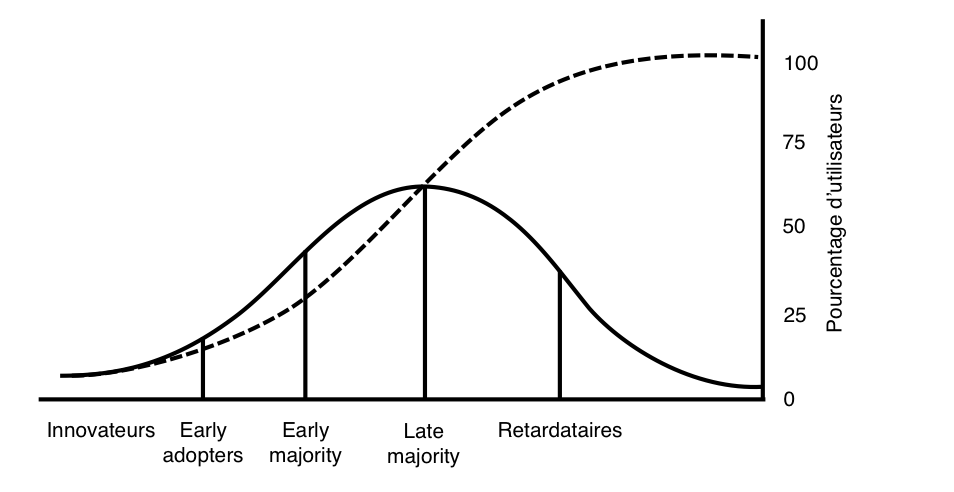
\includegraphics{fig/BassUtilisateurs.eps}
		\end{figure}
		
		Les modèles de diffusion peuvent être résumés dans une seule est même équation différentielle : 
	
			\[
				\dfrac{dN(t)}{dt}=g(t)(m-N(t))
			\]
		
		où $N(t)$ est le nombre cumulé d'individus ayant adopté la technologie à la date t, où $m$ est le seuil maximal du nombre d’acheteurs potentiels, c'est-à-dire la taille du marché, et où $g(t)$ le \textit{coefficient de diffusion}.
		
		
		En fonction de la valeur du coefficient de diffusion g(t), on trouve 3 modèles essentiels :
	
		\begin{enumerate}
			\item modèle des influences externes : $g(t) = p = \text{cste}$.
			Dans ce modèle, le paramètre $p$ peut être interprété comme l’ensemble des facteurs extérieurs qui agissent sur la prise de décision du consommateur (pouvoir des médias et des réseaux sociaux, par exemple) ;
			\item modèle des influences internes : $g(t) = q N(t)$ où $q$ est le \textit{coefficient d’imitation}. Dans ce modèle, le paramètre $q$ représente l’interaction entre les acheteurs potentiels et ceux qui ont déjà adopté la technologie, car pour un futur acheteur l’avis des autres consommateurs est primordial ;
			\item modèle de Bass : $g(t) = p + q \dfrac{N(t)}{m}$. C’est un mélange des deux modèles précédents. Ainsi, sur un intervalle de temps $\Delta t$, le nombre d’individus qui adoptent la technologie est régi par deux phénomènes : 

			\begin{itemize}
				\item contagion, fonction du nombre d’individus ayant déjà adopté l’innovation (terme $q N(t)(m - N(t))$) ;
				\item saturation du fait de la présence du palier $m$.

			\end{itemize}

			La solution à ce problème est :
				\[
					N(t) = \dfrac{m - \dfrac{p (m - N_0)}{p + q \dfrac{N_0}{m}} e^{-(p+q)t}}{1 - \dfrac{\dfrac{q}{m} (m - N_0)}{p + q \dfrac{N_0}{m}} e^{-(p+q)t}}
				\]
				
			avec $N_0 = N(t = 0)$.
		
		\end{enumerate}
		
		Mais tous les modèles précédents supposaient l’existence d’une taille de marché $m$ constante. Cependant, en général, ce n’est pas le cas : on peut considérer l’arrivée de nouveaux conducteurs, les voitures qui parviennent en fin de vie... C’est pour cette raison que l’on adoptera dans notre approche le modèle de Sharif et Ramannathan avec une taille de marché dépendante du temps : $m(t) = m_0 e^{gt}$.
		
		
		La résolution mathématique de ce problème se présente sous cette forme :
		
			\[
				N(t) = m_0 e^{gt} \dfrac{\dfrac{\Phi_1 - \Phi_2}{2} - \Phi_3 \dfrac{\Phi_1 + \Phi_2}{2} e^{-\Phi_1 t}}{q + q \Phi_3 e^{-\Phi_1 t}}
			\]
			
		où $\Phi_1 = \sqrt{(g+p-q)^2 + 4pq}$, $\Phi_2 = g + p - q$ et $\Phi_3 = \dfrac{\dfrac{\Phi_1 - \Phi_2}{2} - q \dfrac{N_0}{m_0}}{\dfrac{\Phi_1 + \Phi_2}{2} + q \dfrac{N_0}{m_0}}$, avec $0 < N_0 \leqslant m_0$.


	\subsection{Utilisation des modèles de diffusion pour le marché du véhicule électrique}

		L'implémentation des modèles précédents pour l'étude du marché des véhicules électriques nécessite la détermination des paramètres $p$, $q$, $N_0$ et $m$ (ou $m_0$ et $g$).

		Pour ce faire, nous utilisons comme données d'entrée le tableau \ref{tab.immatriculeConception} qui est issu de chiffres préfectoraux :
	
		\begin{table}[h!]
			\caption{Nombres mensuels d'immatriculations de véhicules électriques entre janvier 2011 et mars 2015 \label{tab.immatriculeConception}}
			\begin{center}
				\csvautotabular{fig/tableau1.csv}
			
			\end{center}
		\end{table}


		Nous nous intéressons dans un premier temps au modèle classique de Bass, dans lequel le paramètre $m$ ne dépend pas du temps.

		La grandeur $N_0$ se lit directement sur la première ligne du tableau de données : en effet, les nombres d'immatriculations de voitures électriques sont extrêmement faibles avant janvier 2011 et le volume de ces véhicules peut être considéré comme négligeable. Nous prenons donc $N_0 = 100$.

		Les autres paramètres s'obtiennent par utilisation de la méthode OLS qui nous a paru la plus appropriée, et la plus fidèle. Le tracé de $X(t) = N(t) - N(t-1)$ en fonction de $N(t-1)$ donne la courbe de la figure \ref{fig.courbeXt}
		
		\begin{figure}[h!]
			\caption{Tracé de $X(t)$ en fonction de $N(t-1)$ \label{fig.courbeXt} }
			\begin{center}
				\begin{tikzpicture}
					\begin{axis}[
					height = 8cm,
					width = 15cm,
					axis x line = bottom,
					axis y line = left,
					%title = Tracé de $X(t)$ en fonction de $N(t-1)$
					]
					\addplot[mark = +, draw = blue, smooth] file{fig/courbeXt.txt};
					\addplot[color = red, domain = 0:30000] {-4.55*10^(-7)*x^2+0.0414*x+238.79};
					\end{axis}
				\end{tikzpicture}
			\end{center}
			
		\end{figure}
		
		
		Une courbe polynomiale de second degré $X(t) = \alpha_1 + \alpha_2 N(t-1) + \alpha_3 N(t-1)^2$ s'ajuste au graphique obtenu avec les valeurs suivantes (coefficient $R^2 = 0,49$) :
		
		\begin{align*}
			\alpha_1 &= 238,79\\
			\alpha_2 &= 0,04141\\
			\alpha_3 &= -4,55.10^{-7}
		\end{align*}

		On obtient les paramètres suivants :

		\begin{align*}
			p &= \dfrac{-\alpha_2 + \sqrt{\alpha_2^2 - 4 \alpha_1 \alpha_3}}{2} = 0,0024743185\\
			q &= \dfrac{\alpha_2 + \sqrt{\alpha_2^2 - 4 \alpha_1 \alpha_3}}{2} = 0,0438843185\\
			m &= \dfrac{-\alpha_2 - \sqrt{\alpha_2^2 - 4 \alpha_1 \alpha_3}}{2 \alpha_3} = 96507
		\end{align*}

		L'ordre de grandeur de $m$ paraît cohérent, le nombre de véhicules électriques roulant en 2014 étant d'environ 30000. Ceci nous permet d'obtenir le profil de diffusion de la figure \ref{fig.courbeBass1}, dont la limite est égale à $m = 96507$.

		\begin{figure}[h!]
			\caption{Profil de diffusion selon le modèle de Bass \label{fig.courbeBass1}}
			\begin{center}
				\begin{tikzpicture}
					\begin{axis}[
					height = 8cm,
					width = 15cm,
					axis x line = bottom,
					axis y line = left,
					xlabel = mois,
					ylabel = nombre d'utilisateurs cumulés,
%					title = Profil de diffusion selon le modèle de Bass
					]
					\addplot[mark = none, draw = blue, smooth] file{fig/courbeBass.txt};
					\end{axis}
				\end{tikzpicture}
			\end{center}
			
		\end{figure}


		Ce modèle semble avoir une durée de validité assez faible, puisque le palier $X = m$ est obtenu avant 2025. Essayons donc d'implémenter le modèle plus réaliste de Sharif et Ramannathan, dans lequel la capacité globale du marché $m$ dépend du temps, selon une loi exponentielle : $m(t) = m_0\ e^{gt}$.
		
		Nous reprenons les mêmes coefficients d'innovation $p$ et d'imitation $q$ que précédemment. Il est également logique d'adopter $m_0 = 96507$ puisque $m(t = 0) = m_0$.
		
		Reste enfin à trouver une valeur pour le coefficient $g$. N'ayant aucune méthode à notre disposition pour le déterminer, nous adoptons $g = 0,035$ \footnote{Valeur utilisée dans une étude sur la diffusion de l'accès à Internet, au sein de la population française ; A. Kijek, T. Kijek, \textit{Opérations research and decisions}, \textbf{2010}, 3-4, \textit{53-68}.}.
		
		Le graphe obtenu présenté en figure \ref{fig.SharifRaman}.
		
		\begin{figure}[h!]
			\caption{Profil de diffusion selon le modèle de Sharif et Ramannathan \label{fig.SharifRaman}}
			\begin{center}
				\begin{tikzpicture}
					\begin{axis}[
					height = 8cm,
					width = 15cm,
					axis x line = bottom,
					axis y line = left,
					xlabel = mois,
					ylabel = nombre d'utilisateurs cumulés,
%					title = Profil de diffusion selon le modèle de Sharif et Ramannathan
					]
					\addplot[mark = none, draw = blue, smooth] file{fig/SharifRaman.txt};
					\end{axis}
				\end{tikzpicture}
			\end{center}
		\end{figure}
		
	\subsection{Conclusion}
		
		Les résultats obtenus sont insuffisants. Le premier profil montre une saturation trop rapide, le marché étant supposé de taille fixe $m$ : le point d'inflexion est atteint à $t^* = -\dfrac{1}{p+q} \log{\left(\dfrac{p}{q}\right)} = 62 \text{ mois}$.
		
		En ce qui concerne le deuxième modèle utilisé, le profil obtenu ne correspond pas aux données que nous avions initialement. Le graphe de la figure \ref{fig.diverSharifRam} présente la divergence entre la réalité (courbe en pointillés) et la théorie.
		
		\begin{figure}[h!]
			\caption{Divergence entre la réalité et la théorie de Sharif et Ramannathan \label{fig.diverSharifRam}}
			\begin{center}
				\begin{tikzpicture}
					\begin{axis}[
					height = 8cm,
					width = 15cm,
					axis x line = bottom,
					axis y line = left,
					xlabel = mois,
					ylabel = nombre d'utilisateurs cumulés,
%					title = Divergence entre la réalité et la théorie de Sharif et Ramannathan
					]
					\addplot[mark = none, draw = blue, smooth] file{fig/graphe5.txt};
					\addplot[mark =+, draw = red, only marks] file{fig/graphe4.txt};
					\end{axis}
				\end{tikzpicture}
			\end{center}
		\end{figure}
		
		
		De plus, la taille n'est pas illimitée comme le laisserait supposer l'exponentielle $m(t)$ : en réalité, $m$ augmente par paliers, correspondant par exemple aux innovations technologiques... Le temps caractéristique $\tau$ est de 29 mois, ce qui donnerai un modèle valable jusqu'en 2020 environ.
		
		L'extrapolation du premier profil (figure \ref{fig.extraBass}) jusqu'en janvier 2025 nous permet de supposer un nombre d'utilisateurs de véhicules électriques de $N = 163 000$ environ. Nous conservons ce chiffre pour l'étude qui suivra.
		
		\begin{figure}[h!]
			\caption{Extrapolation à partir du modèle de Bass \label{fig.extraBass}}
			\begin{center}
				\begin{tikzpicture}
					\begin{axis}[
					height = 11cm,
					width = 15cm,
					axis x line = bottom,
					axis y line = left,
					xlabel = mois,
					ylabel = nombre d'utilisateurs cumulés,
%					title = Extrapolation à partir du modèle de Bass
					]
					\addplot[mark = none, draw = blue, smooth] file{fig/courbeBass.txt};
					\addplot[mark=none, ycomb, color = red] plot coordinates{(169,169*1101-22438)};
					\addplot[color = red, domain = 22438/1101:169]{1101*x -22438};
					\end{axis}
					\end{tikzpicture}
			\end{center}
		\end{figure}
		
		\clearpage
		
		
% % % % % % % % % % % % % % % % % % % % % % % % % % % % % % % % % % % % % % % % % % % % % % % % % % % % % % % % % % % % % % %

\section{Mod\'elisation num\'erique}
	\subsection{Motivations et objectifs}
		\subsubsection{Motivations}
			En parallèle de notre étude de la diffusion du véhicule électrique, nous avons travaillé sur le modèle permettant d'évaluer l'impact futur des véhicules électrique sur la consommation globale d’électricité. L'usage de l'outil informatique nous semblant essentiel pour une telle modélisation, étant donné le nombre important de paramètres et la taille de nos échantillons de calculs. Nos efforts se sont donc tournés vers l'élaboration d'un algorithme de calcul capable de produire une courbe représentant la puissance nécessaire à la recharge d'un véhicule électrique au cours du temps.

			En répétant cet algorithme pour un nombre donné de véhicules, et en sommant les puissances calculées, on obtient ainsi une courbe de charge globale pour cette flotte.

			Cette production visuelle nous a semblé la plus à même d'être exploitée dans le cadre de notre étude. Un excés de précision n'aurait pas eu de sens, étant donné la nature statistique de nos données, et les différentes approximations et extrapolations effectuées.

		\subsubsection{Objectifs}
			
			Les objectifs principaux de notre travail de modélisation sont donc :
			
			\begin{enumerate}
				\item Produire un résultat visuel et facilement exploitable de la charge imposée au réseau par une flotte de véhicules électrique, flotte la plus représentative possible de la réalité (Modèle de véhicule, utilisation, ...) 
				\item Permettre de modifier aisément certains paramètres du modèle comme la taille de l'échantillon ou les hypothèses de flexibilité (SmartGrid, Vehicule to grid).
				\item Présenter un algorithme et un cheminement logique clair et détaillé, pour permettre une réutilisation ou une adaptation ultérieure aisée.
			\end{enumerate}

			Nous nous sommes donc rapidement attachés à développer une structure et un organigramme du code assez précis. Ainsi même si des contingences techniques apparaissaient et retardaient notre production d'un programme fonctionnel, et donc de courbes résultats, notre travail pourrait tout de même être une base suffisamment claire et modulaire pour une exploitation future.

	\subsection{Cheminement de pensée}
	
		Après un premier algorithme naïf et peu exploitable, présenté dans le rapport intermédiaire, nous avons choisi d'aborder le problème différemment.
		Pour notre modèle final nous avons décidé de travailler avec une approche plus atomique. Nous avons en effet choisi de considérer les véhicules individuellement, et définis de manière indépendante ---  au lieu d'un véhicule moyen ---  et de faire évoluer chaque véhicule pendant la durée de la simulation selon ses caractéristiques propres.
		
		Cela nous a permis de définir nos véhicules avec une cohérence physique plus grande que lors de l'étude d'un véhicule moyen; par exemple l'utilisation de distributions probabilistes dans l'affectation de certains paramètres permet de simuler le comportement individuel aléatoire d'un véhicule réel.

		Le suivi d'un grand nombre de ces véhicules, permet ensuite d'obtenir une courbe moyenne de consommation pour une flotte.
		
		Cette méthode probabiliste de définition des véhicules s'apparente à une approche de type Monte-Carlo, ou le loi des grands nombres justifie l'utilisation de paramètres aléatoires de loi adaptées pour modéliser des systèmes dont la résolution déterministe est impossible.
		
		Une fois notre approche globale définie nous avons été amenés à préciser les paramètres à étudier et à prendre en compte dans notre modèle. En effet la définition de ces paramètres et leurs dépendances allaient fortement conditionner la manière dont l'algorithme et le code seraient structurés.

		Les paramètres retenus sont donc issus d'un travail en amont, et leur définition a été progressivement affinée au fur et à mesure de l'élaboration du modèle. 

	\subsection{Hypothèses et paramètres}
		
		\paragraph{Hypothèses de base.}
		Tout d'abord, il est important de noter que nous n'avons travaillé que dans le cadre d'une journée de semaine non chômée, avec des véhicules effectuant pour l'essentiel des trajets domicile-lieu de travail. Ce choix de situation, comme nombre des autres hypothèses présentées plus bas, s'est imposé a nous pour des questions de simplicité de modélisation. De plus il nous a semblé le plus représentatif d'une situation réelle.
		
		Afin de représenter les déplacements du véhicule, nous avons retenu trois lieux de stationnement où l'utilisateur est susceptible d'utiliser une borne de recharge :
		\begin{itemize}
			\item Sa maison ;
			\item Son lieu de travail;
			\item La voie publique, qui regroupe toutes les autres destinations possibles (centre commercial, centre ville, école des enfants, lieu de loisir, etc.).
		\end{itemize}
		
		Nous avons aussi considéré quatre états de mouvements possible pour un véhicule : 
		\begin{itemize}
			\item En train de rouler : le véhicule se déplace;
			\item Garé non branché  : le véhicule est à l'arrêt et n'est pas relié à une borne de recharge;
			\item Branché en charge  : le véhicule est à l'arrêt, relié à une borne, et se recharge;
			\item Branché par en charge : le véhicule est à l'arrêt, relié à une borne, mais ne se recharge pas (par utilisation d'une recharge différée, ou parce que le véhicule est pleinement chargé).
		\end{itemize}
		
		
		\paragraph{Paramètres physiques.} Nous avons retenu cette liste de paramètres physiques caractérisants nos véhicules :
		
		\begin{itemize}
			\item Le type de véhicule, à savoir : Véhicule particulier (VEP), Véhicule d'entreprise (VEE), ou Véhicule d'auto partage (VAP);
			\item Le modèle de véhicule : nous en avons retenus 5 différents (Renault Zoé, Nissan Leaf, Bolloré Blue Car, Smart ForTwo et Tesla Model S);
			\item La capacité de la batterie du véhicule (en \si{\kilo\watt\hour}) et la consommation (en \si{\kilo\watt\hour\per\kilo\meter}), dépendant directement du modèle de véhicule;
			\item La vitesse : supposée constante pour chaque véhicule, elle est initialisée pour chaque véhicule à partir d'une distribution gaussienne centrée à \SI{38,75}{\kilo\meter\per\hour}, valeur moyenne pour les déplacements des véhicules en France, et un écart type de 10.
			\item La longueur d'un trajet : de même que pour la vitesse, nous effectuons l'hypothèse que pour un véhicule donné, tous ses trajets font la même longueur. Cette longueur est tirée selon la répartition statistique des distances parcourues par les véhicule en France;
			\item Le nombre de trajets effectués en une journée : de même que pour les deux paramètres précédents, chaque véhicule effectue un nombre de trajet fixe, initialisé selon une distribution gaussienne, dont les paramètres sont issus des données statistiques à notre disposition;
			\item L'accès aux bornes : chaque véhicule a éventuellement à sa disposition une borne au différentes positions possibles (ex : le VEP n°1 possède une borne chez lui, mais ni au travail, ni dans les lieux public qu'il fréquente, tandis que le VEP n°2 possède une borne chez lui, et également sur son lieu de travail ou son employeur a mis en place des bornes a disposition des employés). Cette répartition est issue de données statistiques à priori, mais peut être modulée pour générer des projections dans divers cas futurs.  
			\item L'état de charge (State of Charge ou SOC) : évoluant au cours du temps, évalué en pourcentage de la capacité totale de batterie;
			\item L'état de mouvement du véhicule et sa position, tels que définis ci-dessus;
			\item Les horaires de trajets du véhicule : à partir de données statistiques sur les horaires de trajets réels, et du nombre de trajets qu'il va effectuer, chaque véhicule se voit affecter une liste d'horaires à laquelle il est censé partir de sa position actuelle (s'il est insuffisamment chargé il attendra le temps nécessaire à sa recharge).
		\end{itemize}
		
		Dans cette liste de paramètres apparaissent déjà un certain nombre d'hypothèses, qui peuvent sembler assez fortes, sur la définition d'un véhicule : vitesse et longueur des trajets fixes ou encore horaires des trajets définis à l'avance et pour toute la durée de la simulation.
		
		Ces hypothèses nous ont semblé nécessaires pour pouvoir créer un algorithme d'une complexité raisonnable. De plus ces écarts à la réalité physique d'un véhicule sont compensés par l'utilisation d'un grand nombre de véhicules de paramètres aléatoires lors des modélisations. Comme les variables aléatoires sont choisies en adéquation avec les données statistiques réelles, la loi des grands nombre assure la convergence de nos simulations avec des véhicules virtuels vers les valeurs attendues dans la réalité.
		
		\paragraph{Hypothèses supplémentaires.} A ce qui a été présenté précédemment nous avons ajoutés un certain nombre de variables et d'hypothèses qui ont un sens physique, mais dont les définitions relèvent plus de l'arbitraire et du \emph{qualified guess} que de données statistiques. Tous ces paramètres font partie de la définition d'un véhicule et même si certains évoluent au cours de la simulation l
		
		\begin{itemize}
			\item Les destinations des véhicules sont choisies a priori. 
				\begin{itemize}
				
					\item Pour un VEP nous avons considéré divers cas horaires :
					\begin{itemize}
						\item de 7h à 11h tous les trajets d'un particulier le conduise sur son lieu de travail, et dans le cas ou il est déjà sur son lieu de travail un trajet l’amène dans un lieu public (déplacement professionnel);
						\item de 11h à 14h un trajet depuis un lieu public (ou il a pris son repas par exemple) l'amène sur son lieu de travail, et un trajet depuis sa maison ou son lieu de travail l'amène aléatoirement à l'un des deux autres lieu possibles (trajet travail->maison pour le repas par exemple, ou maison->lieu extérieur pour aller chercher les enfants à l'école);
						\item de 0h à 7h et de 14h à 24h un trajet depuis la maison l'amène sur un lieu public (école des enfants, sortie le soir, courses, etc.), et tout autre trajet a pour direction la maison.
					\end{itemize}
					
					\item Pour un VEE il y a aussi une distinction horaire, mais plus simple :
					\begin{itemize}
						\item s'il est plus de 18h le véhicule rentre sur son lieu de travail, qui dans le cas d'un véhicule d'entreprise est sa base de départ;
						\item sinon tous les déplacements sont des déplacements professionnels qui vont vers un lieu public.
					\end{itemize}
					
					\item Enfin pour un véhicule d'auto-partage le trajet est aléatoirement vers un lieu public, ou un lieu de travail.
				\end{itemize}
			Ces destinations sont déterminées lors de l'initialisation d'un véhicule, et un parcours de ce tableau vérifie que chaque véhicule accède à une borne au cours de ses trajets, quitte à recommencer la création du véhicule si celui-ci ne trouve pas de bornes sur son trajet.
			\item Nous avons imposés certaines contraintes sur la répartition des bornes des VEE et VAP :
				\begin{enumerate}
					\item Un VEE aura toujours une borne sur son lieu de travail;
					\item Un VAP aura toujours une borne disponible dans un lieu public (nous faisons l'assomption que l'utilisateur le ramène toujours près d'une borne après utilisation).
				\end{enumerate}
			\item Pour prévenir la "panne sèche" d'un véhicule au cours d'un trajet, nous avons introduit une variable \texttt{socMin} qui contient l'état de charge minimum requis pour voyager jusqu’à la prochaine borne. Le calcul de cette variable est simplifié par la connaissance au préalable des destinations, de l'accès au bornes et de la distance des trajets. Cela peut paraitre un peu artificiel dans le cadre de notre modèle, mais dans la réalité un utilisateur a la plupart du temps connaissance de ses capacités de recharge au cours du trajet, et les prends en compte lorsqu'il débranche ou non son véhicule. Nous supposons que le véhicule ne peut redémarrer s'il n'a pas atteint un état de charge supérieur ou égal a \texttt{socMin}. 
			
		\end{itemize}

	\subsection{Description de l'algorithme}
		
		L'algorithme se décompose donc en deux parties distinctes :
		\begin{enumerate}
		
			\item Tout d'abord l'initialisation du véhicule, qui doit définir tous les paramètres décrits ci-dessus, et s'assurer que ceux ci caractérisent un véhicule fonctionnel, c'est à dire un véhicule qui a accès à des bornes, qui peut faire tous ses trajets, etc. Cette partie est organisée de manière très linéaire, avec une succession d'affectation et de vérifications qui aboutissent à la définition du véhicule. Elle est effectuée une fois par véhicule. Sa structure est détaillée au paragraphe \ref{sec.descrInit}
			
			\item Ensuite la partie d'évolution. Elle consiste essentiellement en une série de tests sur l'état du véhicule (quel est son état de mouvement, son état de charge, le nombre de trajets à effectuer, etc) qui modifient ces mêmes paramètres d'état selon les résultats obtenus. C'est une boucle que chaque véhicule parcours une fois par pas de temps. C'est dans cette partie que va être modifié le tableau résultat \texttt{puissanceReseau}, qui contient la puissance nécessaire à la recharge de la flotte considérée pour chaque pas de temps. La structure de cette boucle est illustrée par les diagrammes \ref{fig.flowPrincipal} et \ref{fig.flowTransition}, et commentée dans le paragraphe \ref{sec.descrSimulation}.
		
		\end{enumerate}
		
		\subsubsection{Initialisation des véhicules \label{sec.descrInit}}
			
			Comme mentionné ci-dessus, l'initialisation des véhicule est un processus séquentiel, où l'ordre des étapes dépend de manière fondamentale des dépendances entre les paramètres. Une partie importante de sa conception a donc été de bien distinguer ces dépendances pour pouvoir écrire un programme ayant du sens physiquement, et avec des étapes les plus élémentaires possibles.
			
			Voici donc les étapes de l'initialisation d'un véhicule :
			
			\begin{enumerate}
				\item Initialisation du SOC (\texttt{soc}) à 100 $\percent$ : ab initio tous les véhicules sont chargés.
				\item L'état de mouvement (\texttt{etatMouvActuel}) est défini comme branché en charge (\texttt{BRANCHE\_EN\_CHARGE}).
				\item L'état de mouvement suivant, variable interne utilisée dans la boucle d'évolution, est défini de même : \texttt{etatMouvSuivant = BRANCHE\_EN\_CHARGE}.
				\item Initialisation de la distance parcourue et du nombre de trajets effectués par le véhicule à 0 : \texttt{distanceParcourue = 0; nbTrajetsEffectues = 0}.
				\item Initialisation du type de véhicule (\texttt{typeVehicule}) : VEE, VAP ou VEP.
				\item Initialisation de la position (\texttt{position}) de départ du véhicule.
				\item Définition du modèle du véhicule (\texttt{modele}).
				\item Initialisation de la capacité et de la consommation du véhicule, qui dépendent du modèle de véhicule (\texttt{consommation}, \texttt{capacite}).
				\item Initialisation de la vitesse de déplacement et de la longueur des trajets tels que présentés plus hauts (\texttt{vitesse},\texttt{longueurTrajet}).
				\item Initialisation du nombre de trajet par jour (\texttt{nbTrajets}).
				\item Disponibilité des bornes : maison OUI/NON, lieu de travail OUI/NON, lieu public OUI/NON. (tableau \texttt{accesBornes}).
				\item Test de la disponibilité d'au moins une borne pour le véhicule.
				\item Calcul des horaires de départs (\texttt{horaireDepart})
				\item Vérification qu'il n'y a pas chevauchement entre un trajet et le suivant, c'est à dire que le véhicule à bien fini le trajet précédent au moment ou il doit effectuer le suivant.
				\item Vérification que le véhicule passe bien par une borne au cours de la journée.
				\item Initialisation du SOC minimal (\texttt{socMin}) à la valeur nécessaire pour atteindre la prochaine borne.
			\end{enumerate}	
	
			Cette initialisation correspond au constructeur \texttt{Vehicule::Vehicule(int deltaT)} de la classe \texttt{Vehicule.cpp}. Le paramètre \texttt{deltaT} correspond au pas de temps de la simulation. Une fois le véhicule correctement initialisé nous le faisons évoluer dans la boucle de simulation.
	
		\subsubsection{Boucle de simulation \label{sec.descrSimulation}}
			
			L'organisation logique de la partie évolutive de la simulation est présentée dans le diagramme ci dessous (figure \ref{fig.flowPrincipal}). Pour plus de lisibilité le bloc transition est présenté à part, dans la figure \ref{fig.flowTransition}. Ces deux blocs correspondent respectivement aux méthodes \texttt{double Vehicule::simulation(int temps, int deltaT)} et \texttt{int Vehicule::transition(int temps, int deltaT)} de la classe \texttt{Vehicule.cpp}. L'opération de bouclage de la méthode \texttt{simulation} est effectué lors de son appel dans la fonction \texttt{main}.
			
			La méthode \texttt{simulation} prend en paramètre le \texttt{temps} actuel --- mesuré en nombre de pas de temps \texttt{deltaT} --- et retourne la puissance demandée par le véhicule sur lequel on appelle cette méthode a l'instant \texttt{temps}.
			La méthode \texttt{transition} prend les mêmes paramètres que \texttt{simulation} et retourne un entier correspondant à l'état de mouvement dans lequel sera le véhicule au prochain pas de temps (\texttt{etatMouvSuivant}).
			
			
		
			\begin{figure}[h]
				\centering
				\caption{Logigramme de la méthode \texttt{simulation} \label{fig.flowPrincipal}}
				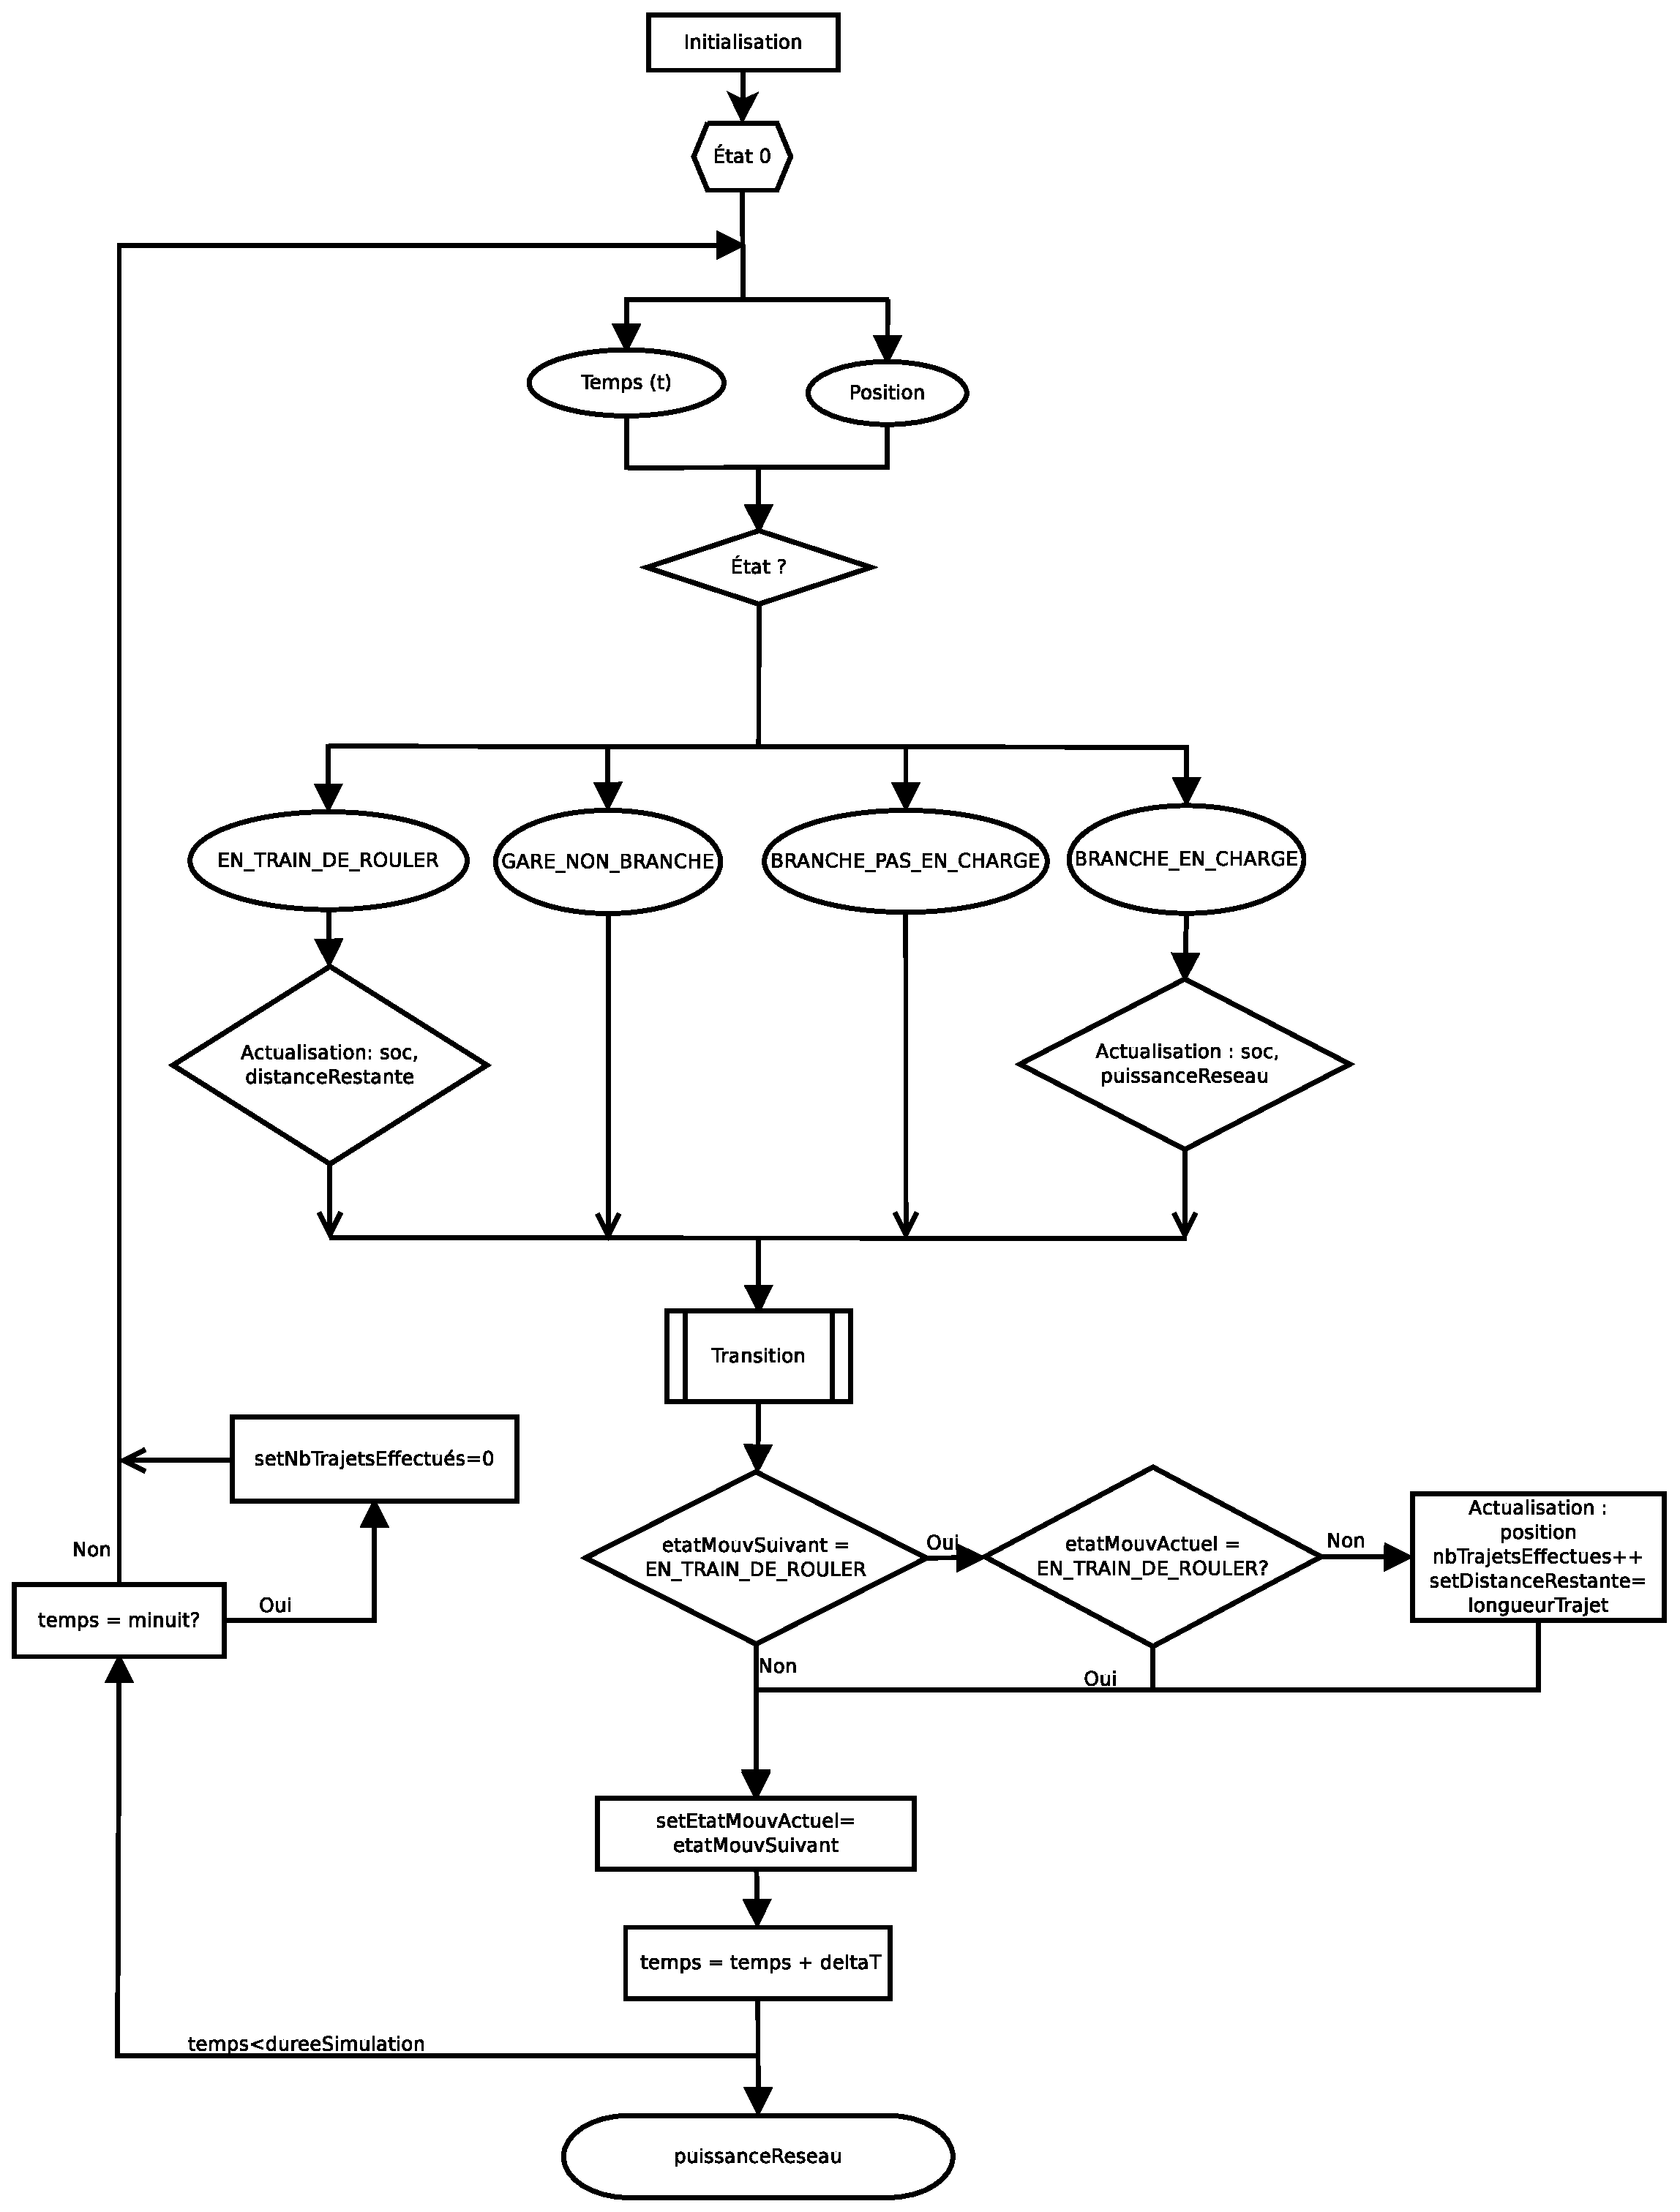
\includegraphics[height=0.9\textheight]{fig/flowPrincipal.eps}
			\end{figure}
			\begin{figure}[h]
				\centering
				\caption{Bloc Transition \label{fig.flowTransition}}
				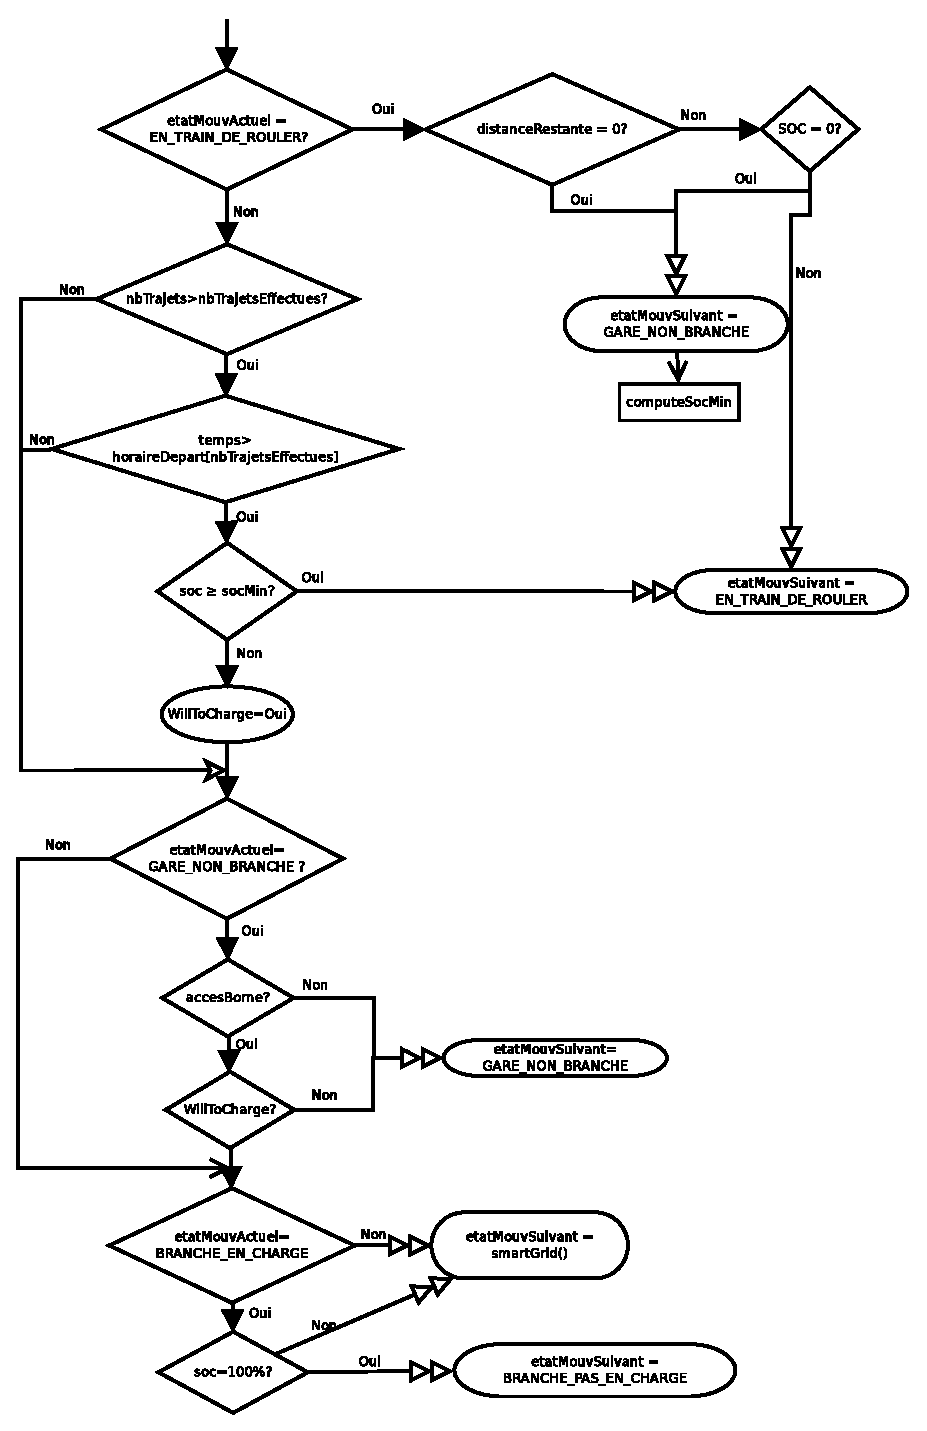
\includegraphics[height=0.9\textheight]{fig/flowTransition.eps}
			\end{figure}
		
		
		\clearpage
	\subsection{Résultat}

2 jours == 10 jours mentionner
 

\end{document}